\chapter{Background}
\label{chap:background:intro}

To motivate the architecture design space introduce in chapter (REFERENCE chapter)
I first need to 
3) show how to convert a convolution operation into a GEMM
4) Introduce dataflow exploration through direct representation if implementing
an accelerates that accelerates convolutions directly
5) Introduce hardware 
+ based on reuse behavior in the Dataflow
dataflow -> describes communication -> describes datareuse
6) Introduce polyhedral model to evaluate temporal reuse behavior
In this chapter I
breakdown what convolutions are mathetmatically


\figref{fig:cnn_network}

\begin{figure}[ht]
    \centering
    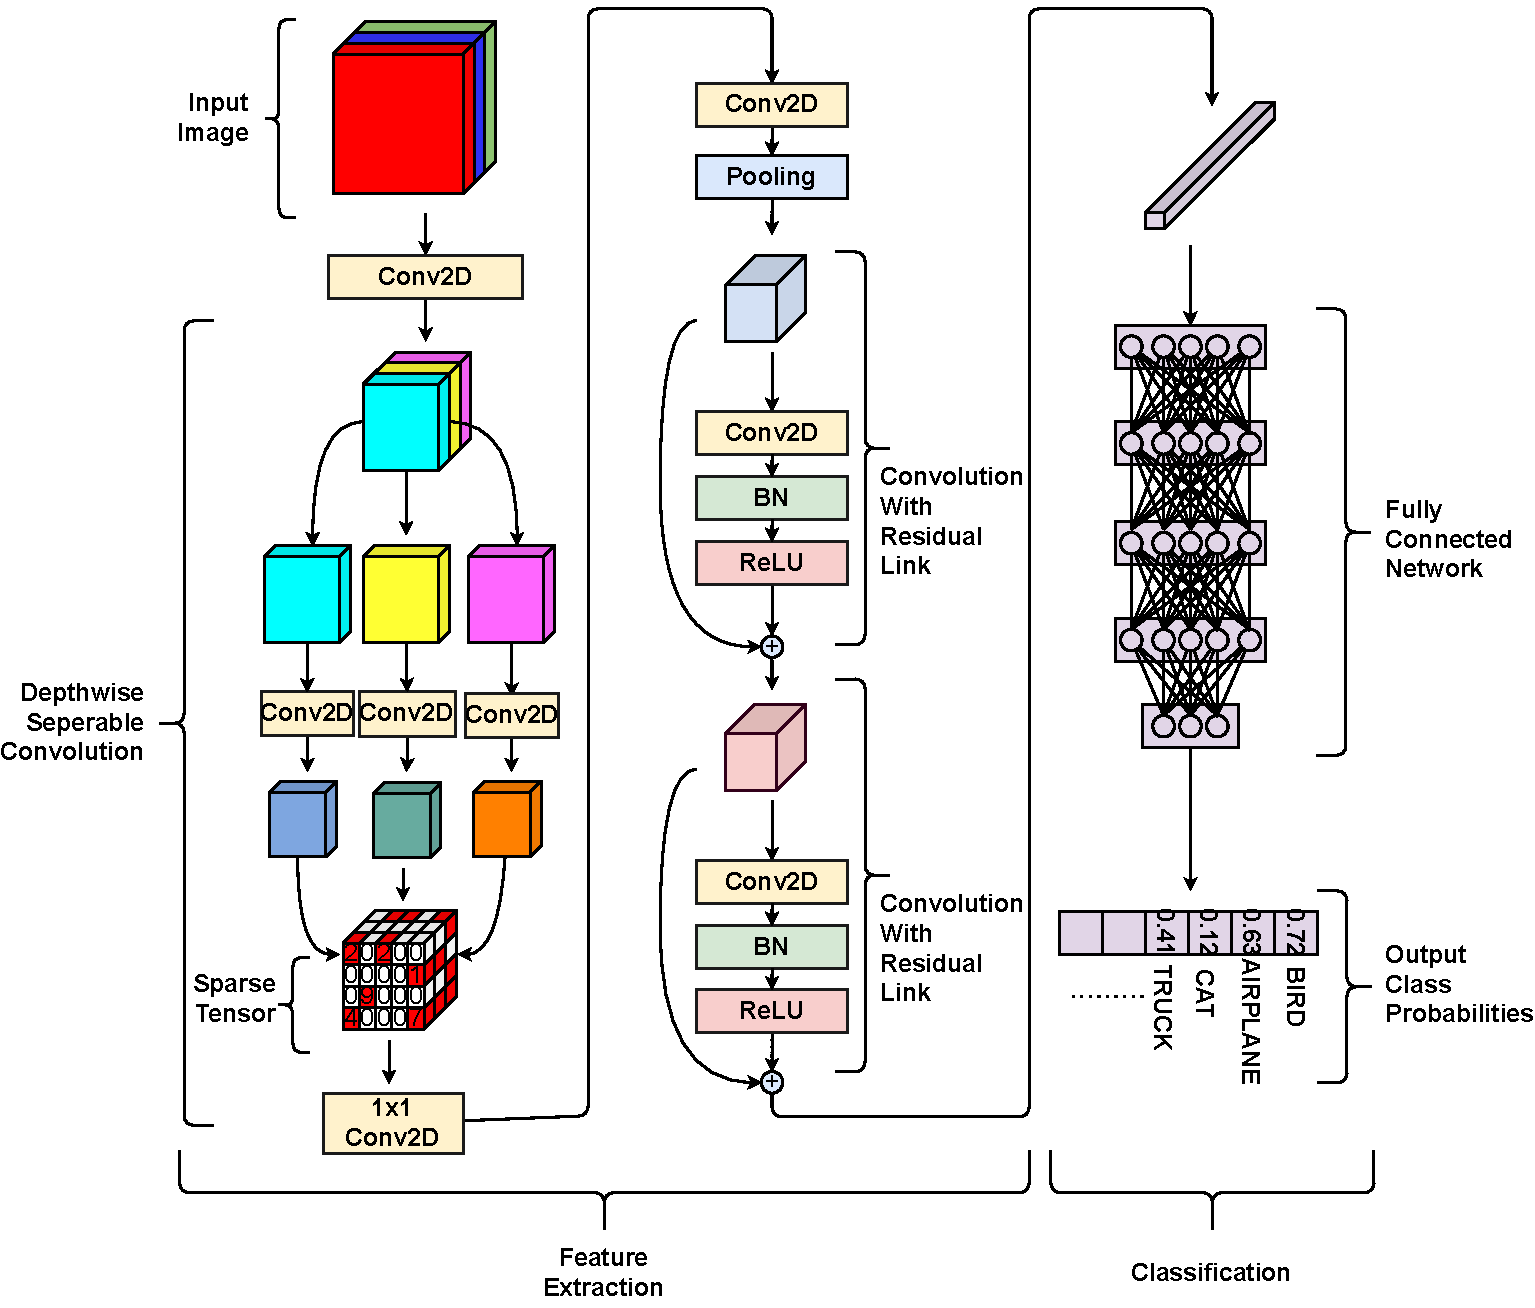
\includegraphics[scale=0.4]{fig/cnn.pdf}
    \caption{Example Image Classfication CNN}
    \label{fig:cnn_network}
\end{figure}

\clearpage

\section{The Math behind convolutions}
\label{chap:intro:conv_operation}

1) explain what convolutions are mathematically

\begin{figure}[ht]
    \centering
    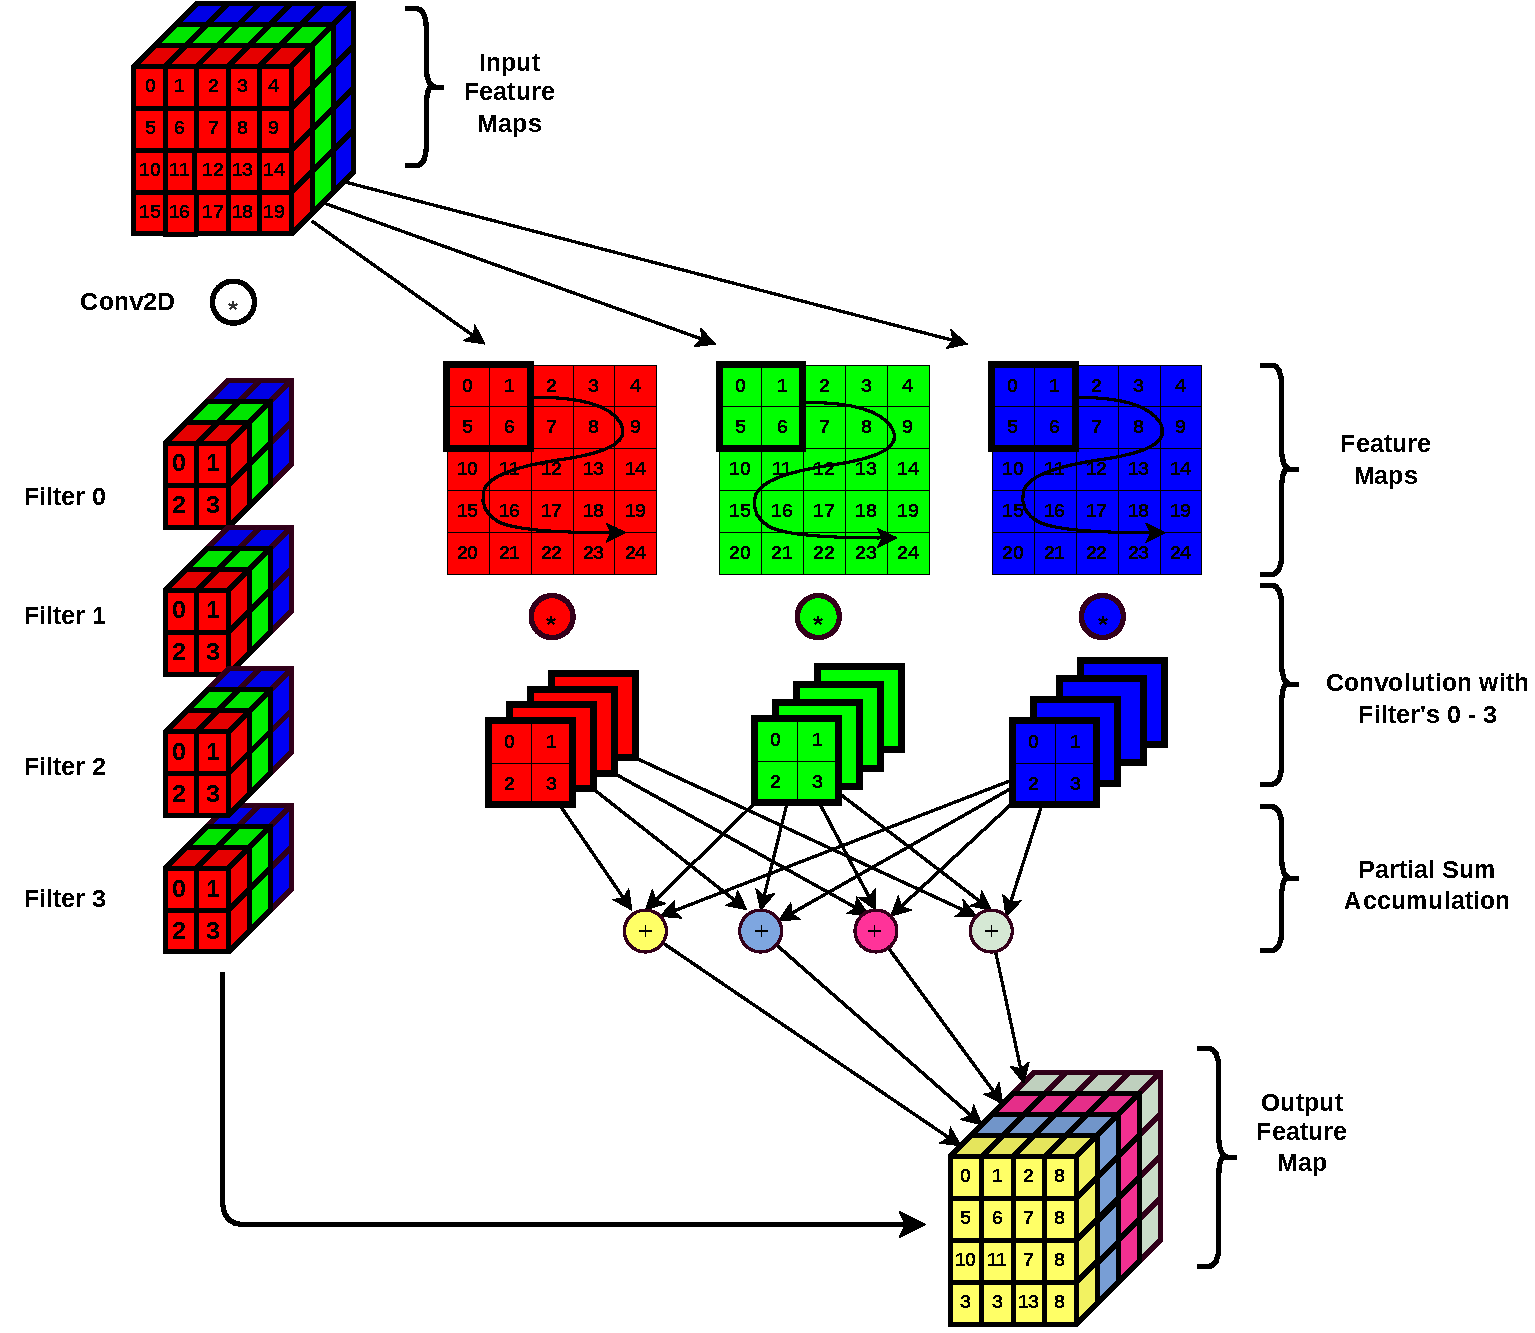
\includegraphics[scale=0.6]{fig/ConvExplained.pdf}
    \caption{Convolution Operation Illustrated}
    \label{fig:conv_explained}
\end{figure}

\begin{align}
    \begin{split}
        IFmap \in R^{C \times n\times n} \\
        OFmap \in  R^{F \times m\times m} \\
        Weight \in R^{F \times C\times K\times K} \\
    \end{split}
    \label{math:default_tensor_def}
\end{align}

\begin{align}
    OFmap[f][y][x] = \displaystyle\sum\limits_{c=0}^{C-1}\displaystyle\sum\limits_{k_x=0}^{K-1}\displaystyle\sum\limits_{k_y=0}^{K-1}Weight[f][c][k_y][k_x]*IFmap[c][y+ky][x+kx]
    \label{math:conv_equation_1fp}
\end{align}

\section{Loop Based Representation Of Convolutions}
\label{chap:intro:conv_operation}

Direct naive implementation of \autoref{math:conv_equation} with tensors
\autoref{math:default_tensor_def} as a series of loops is given below
\autoref{lst:conv_loop}

\begin{minipage}{\linewidth}
    \begin{lstlisting}[language=C, caption=Convolution implemented as nested loops, label={lst:conv_loop}]
for(int f = 0; f < F; f++) // Filter loop
    for(int c = 0; c < C; c++) // Channel loop
        for(int y = 0; y < Y; y++) // Output feature map row
            for(int x = 0; x < X; x++)  // Output feature map col
                for(int ky = 0; ky < KY; ky++)  // Kernel row
                    for(int kx = 0; kx < KX; kx++)  // Kernel col
                        O[f][y][x] += I[c][y+ky][x+kx]*W[f][c][ky][kx];
    \end{lstlisting}
\end{minipage}

\newpage

\section{Convolution as general matrix multiplication}
\label{chap:intro:conv_operation}

\begin{figure}[ht]
    \centering
    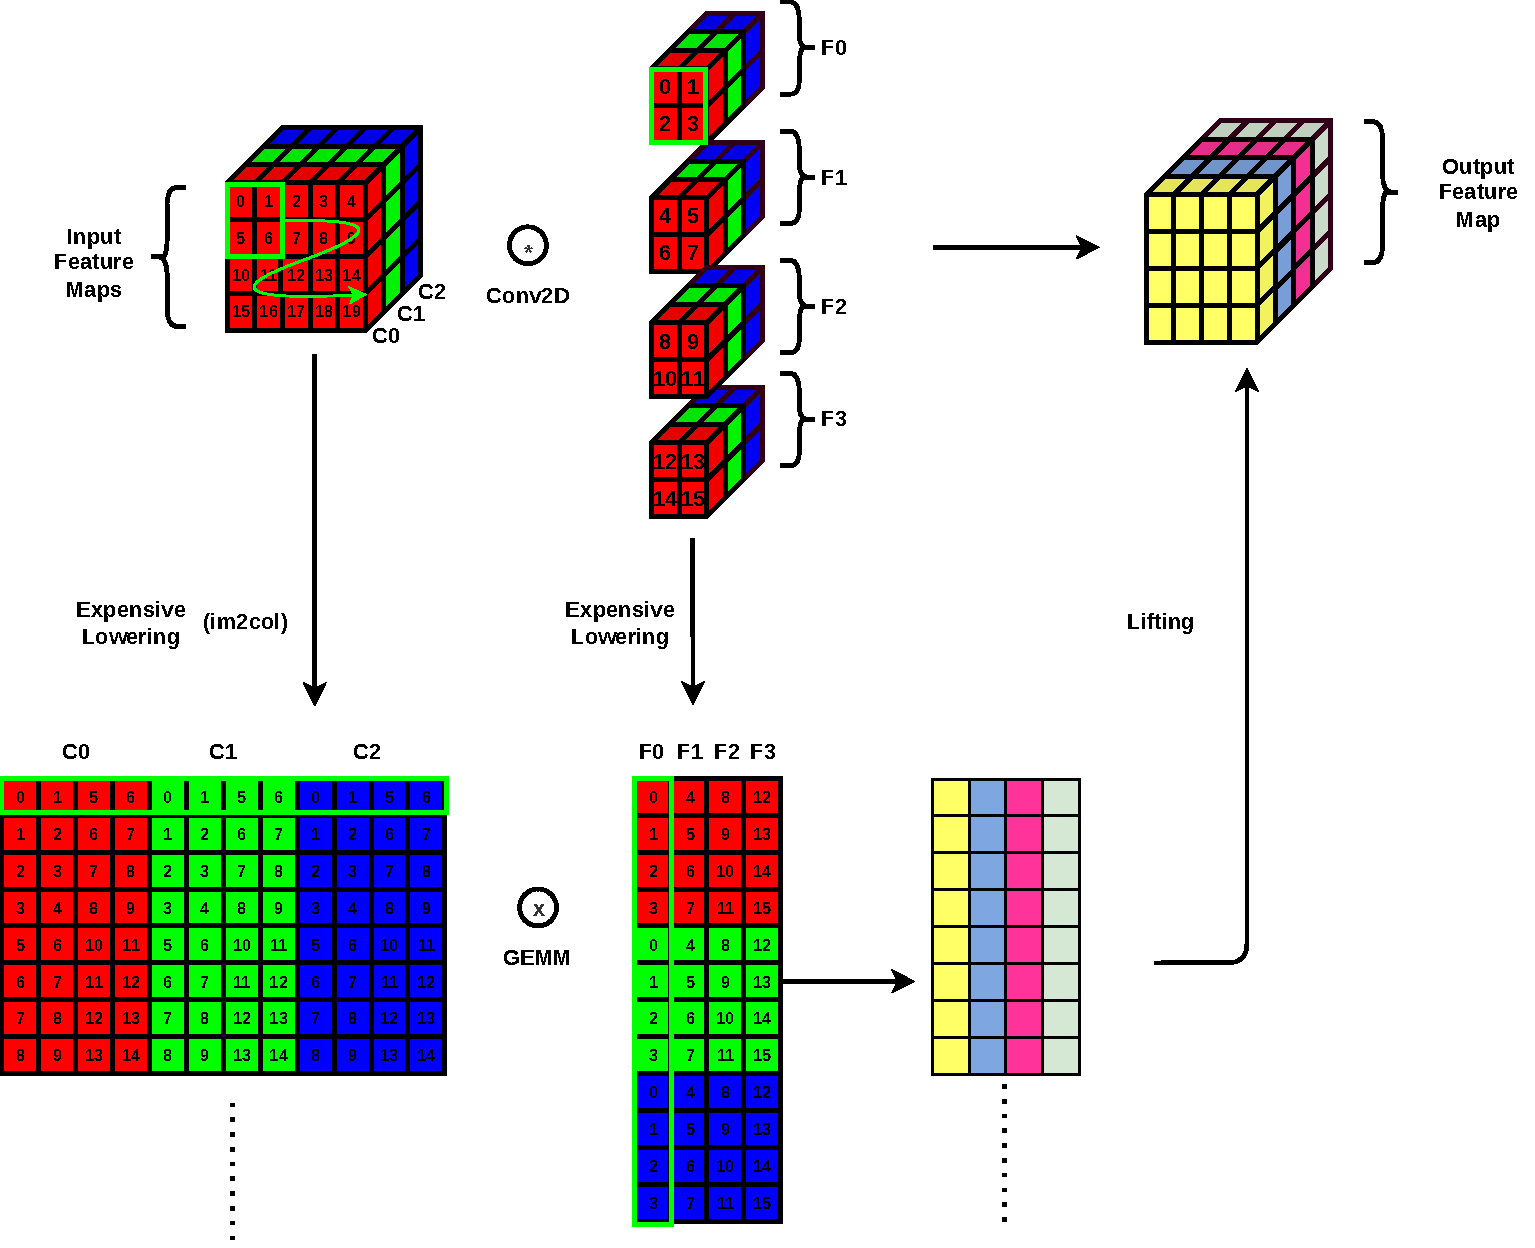
\includegraphics[scale=0.6]{fig/Im2Col.pdf}
    \caption{Im2Col Illustrated}
    \label{fig:im2col}
\end{figure}

Convolution can be converted into a \ac{GEMM}

Popular techniques like im2col (illustrated in \autoref{fig:im2col}) can be used
to convert any convolution operation into \ac{GEMM} (listed as expensive
lowering \cite{cafe_con_troll}) but there are others techniques that don't
produce such massive input feature maps


If willing to increase complexity of lowering of ifmap and weight tensors after
GEMM we can reduce bloat in ifmap with balanced lifting/ loading in
\cite{cafe_con_troll}. Analytical expressions adapted from \cite{cafe_con_troll}
are given below with the inclusion of lowering in the presence of multiple
filters.


\clearpage

\begin{align}
    \begin{gathered}
        IFmap \in R^{C\times n\times n} \xrightarrow[]{Balanced Lowering} \hat{IFmap} \in R^{nm\times KC} \\
        \hat{IFmap}[cn+r, :] = vec(IFmap[:, r, c:c+K]) \\
        \forall r,c \in [0, n-1], [0, m-1]
    \end{gathered}
    \label{math:balanced_lowering_ifmap}
\end{align}

\begin{align}
    \begin{gathered}
        Weight \in R^{F\times C\times K \times K} \xrightarrow[]{Balanced Lowering} \hat{Weight} \in R^{KC\times FK}\\
        \hat{Weight}[f*K:f*K+K, i] = vec(Weight[f, :, i, :]) \\
        \forall f,i \in [0, F-1], [0, K-1]
    \end{gathered}
    \label{math:balanced_lowering_weight}
\end{align}
In balanced lowering, we first lower the ifmap and weights using expression 
\eqref{math:balanced_lowering_ifmap} and \eqref{math:balanced_lowering_weight}.

\begin{align}
    \begin{gathered}
        \hat{OFmap} = \hat{IFmap}.\hat{Weight}
    \end{gathered}
    \label{math:balanced_lowering_gemm}
\end{align}
Then a \ac{GEMM} is performed \eqref{math:balanced_lowering_gemm}


\begin{align}
    \begin{gathered}
        \hat{OFmap} \in R^{nm\times FK} \xrightarrow[]{Balanced Lifting} OFmap \in  R^{m\times m\times F}\\
        OFmap[f, r, c] = (\displaystyle\sum\limits_{j=0}^{K-1} \hat{OFmap}[cn+r+j, j+fK]) \\
        \forall f,r,c \in [0, F-1], [0, m-1], [0, m-1]
    \end{gathered}
    \label{math:balanced_lifting_ofmap}
\end{align}

Followed by a lift operation on the output $\hat{OFmap}$ matrix using \eqref{math:balanced_lifting_ofmap}

Illustration of this data transformation is presented in \autoref{fig:balanced_lowering_lifting}

Pros of lowering/ lifting

Conv as GEMM Offers the most flexibility because it’s insensitive to changes in
convolution parameters

It also allows leaves us with a GEMM accelerator which is useful for many other
NN layers e.g Linear/ Self attention/ LSTM

Con is that it still causes bloat in ifmap and additionaly complexity/ latency of 
lifting/ lowering. Which in the balanced case is $m^{2}K$ \cite{cafe_con_troll}

\begin{figure}[!ht]
    \centering
    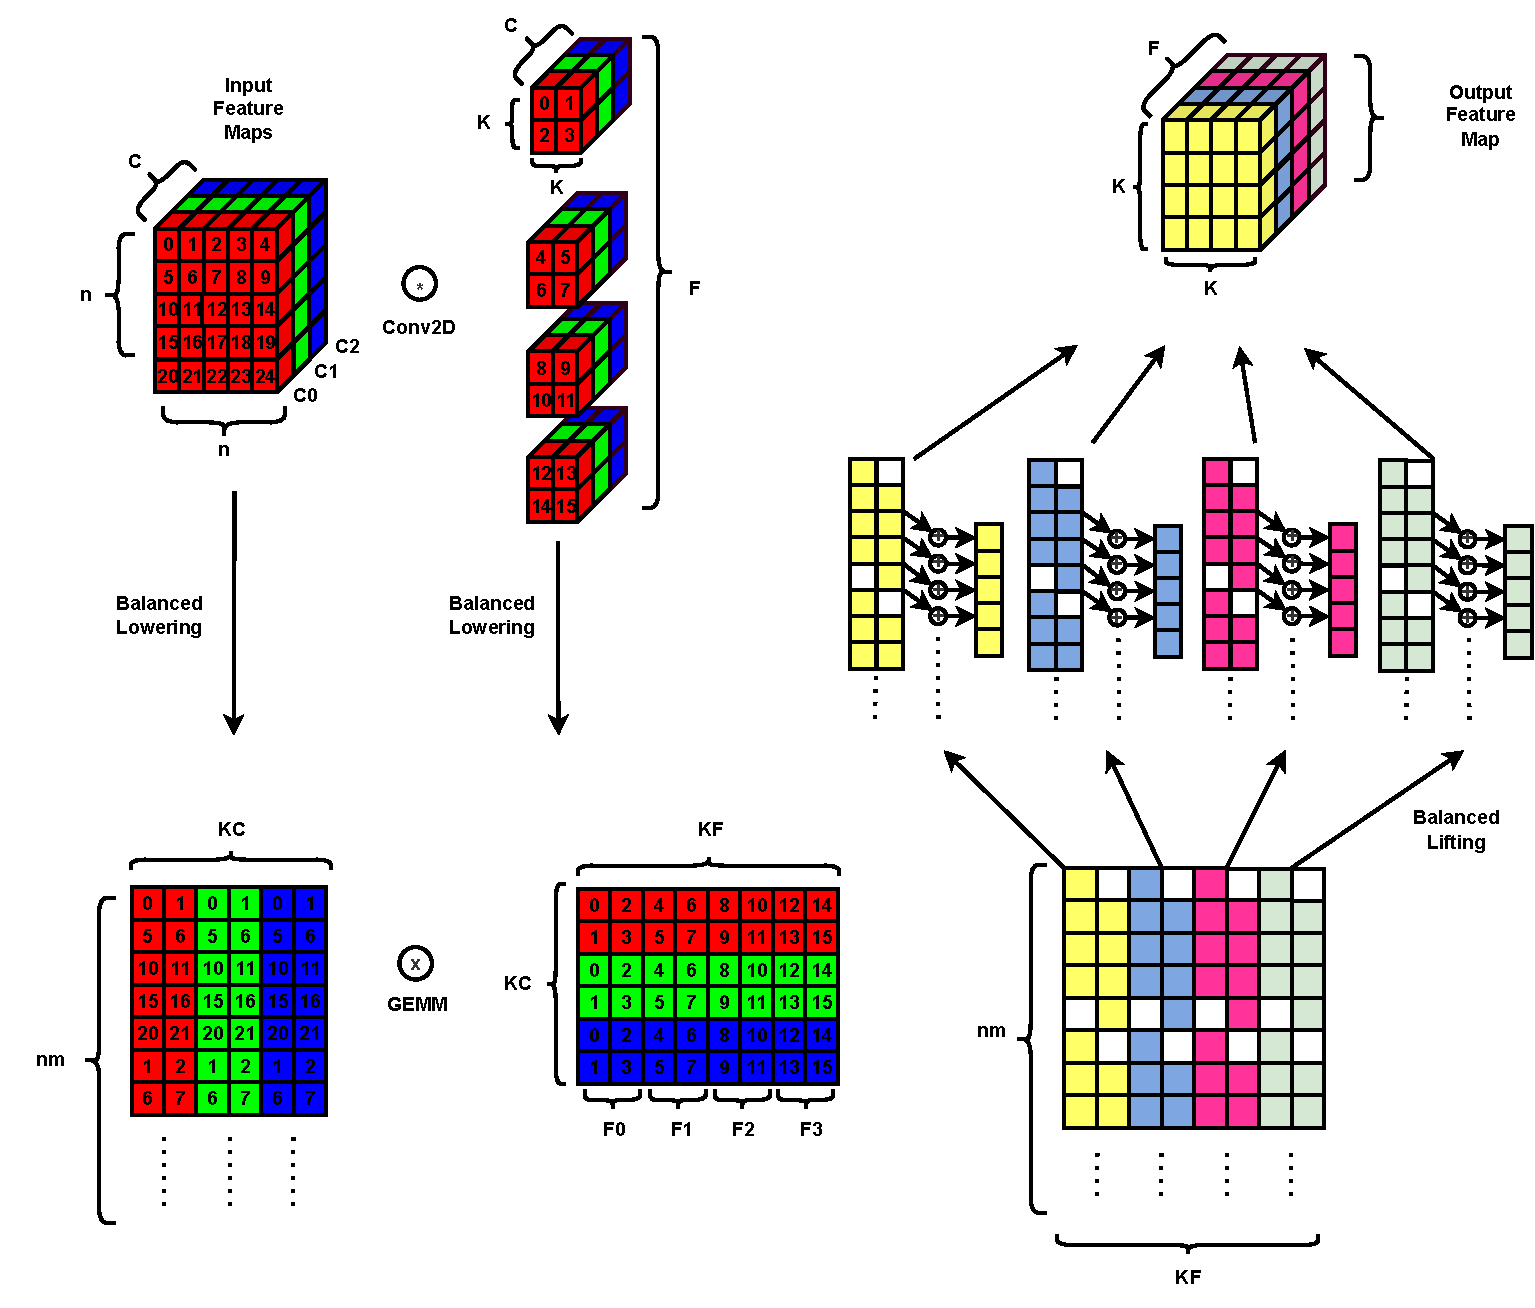
\includegraphics[scale=0.6]{fig/BalancedLoweringLifting.pdf}
    \caption{Balanced Lowering/Lifting Illustrated}
    \label{fig:balanced_lowering_lifting}
\end{figure}


\section{Implementing convolutions in hardware}
\subsection{The dataflow taxonomy}

In the dataflow design space, from \cite{dnn_df_overrated} 
dataflows can be represented using the direct convolution
nested loop structure combined with unroll pragmas. Listing \ref{lst:W_S_Generic_Loop} shows a generic
implementation of a single convolution layer as a loop structure under a weight
stationary dataflow configuration. What defines that dataflow is 1) loop unroll
targets 2) loop order 3) the unroll factors of the unrolled loops. Weight elements within a
kernel remain stationary throughout the computation of an output feature map
until a new tile of channels C\_T is loaded into the accelerator. Once the
weights within a particular channel and filter group are used to produce an
output feature map they are discarded and are only loaded again when computing
the same layer for a new input image. From listing \ref{lst:W_S_Generic_Loop} we
can see that from the loop unroll targets and loop unroll factors there are many
other possible dataflow configurations available to us outside of weight
stationary. Additionally, since accelerators are generally limited to two
spatial axis the loops of the convolution operation can be mapped to two spatial
axis. If we allow multiple convolution loops under some kernel unroll factor
KY\_T/KX\_T  to be unrolled and mapped to the same accelerator spatial axis we
can influence the effective unroll factors when performing different
convolutions of different kernel sizes other than KY\_T/KX\_T. The choice of
which loops are mapped to which spatial axis is an additional design dimension
alongside loop unrolling. To summarize, from the loop representation of
convolution accelerator dataflows we have three design space dimensions, 1) Loop
unroll targets 2) Loop unroll factors 3) Loop spatial mapping. Given the size of
this dataflow design space we will use CIGAR and Tempo to derive the common
case for convolution layers and limit the scope of the dataflow design space.

CNN layer loops + loop ordering + Loop tilings can express different
accelerators dataflows like row stationary, weight stationary, etc



\begin{minipage}{\linewidth}
    \begin{lstlisting}[language=C, caption=Convolution implemented as nested loops, label={lst:conv_loop}]
#pragma UNROLL F_T
for(int f = 0; f < F; f+=F_T) // Filter loop
#pragma UNROLL C_T
    for(int c = 0; c < C; c+=C_T) // Channel loop
#pragma UNROLL Y_T
        for(int y = 0; y < Y; y+=Y_T) // Output feature map row
#pragma UNROLL X_T
            for(int x = 0; x < X; x+=X_T)  // Output feature map col
#pragma UNROLL KY_T
                for(int ky = 0; ky < KY; ky+=KY_T)  // Kernel row
#pragma UNROLL KX_T
                    for(int kx = 0; kx < KX; kx+=KX_T)  // Kernel col
                        O[f][y][x] += I[c][y+ky][x+kx]*W[f][c][ky][kx];
    \end{lstlisting}
\end{minipage}


\begin{figure}
    \centering
    \subfigure[]{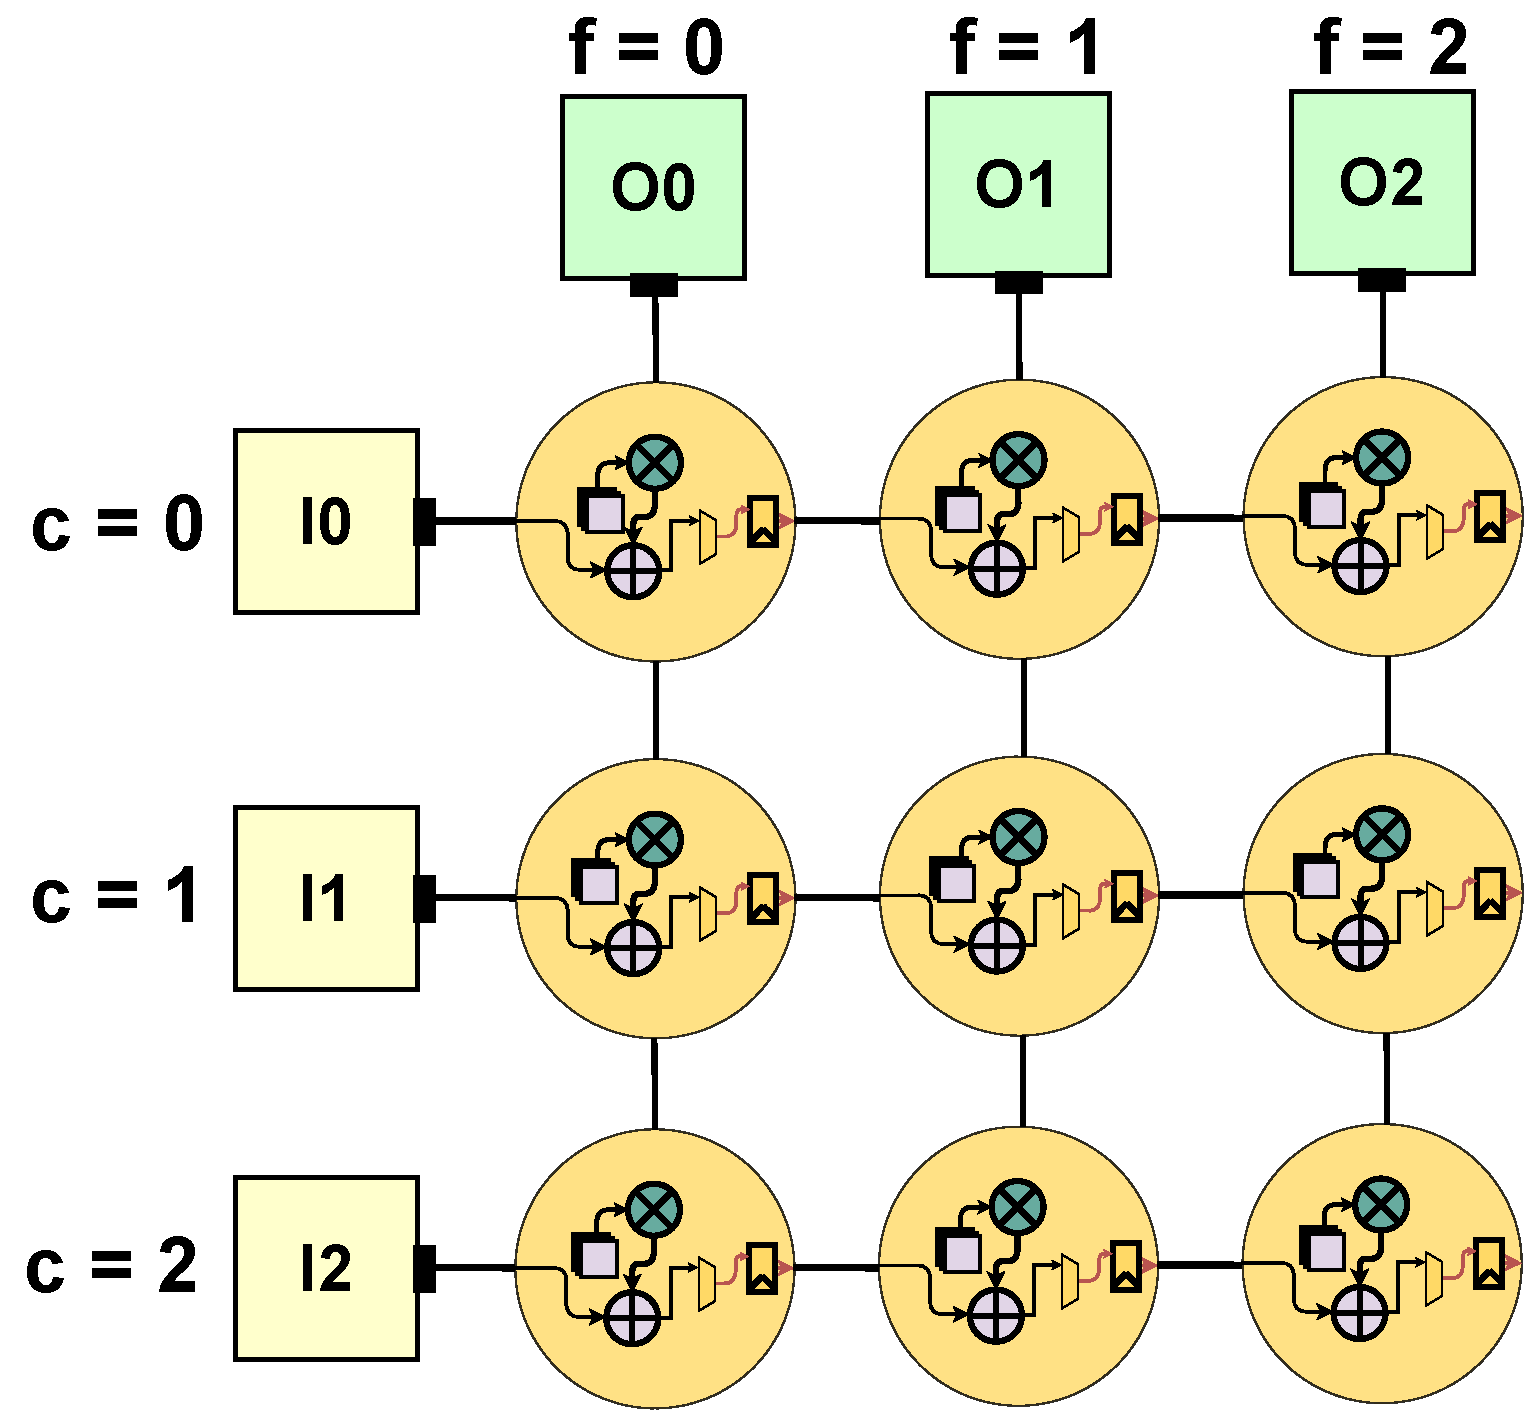
\includegraphics[width=0.32\textwidth]{fig/unroll_c_f.pdf}}
    \hspace{0.1cm} 
    \subfigure[]{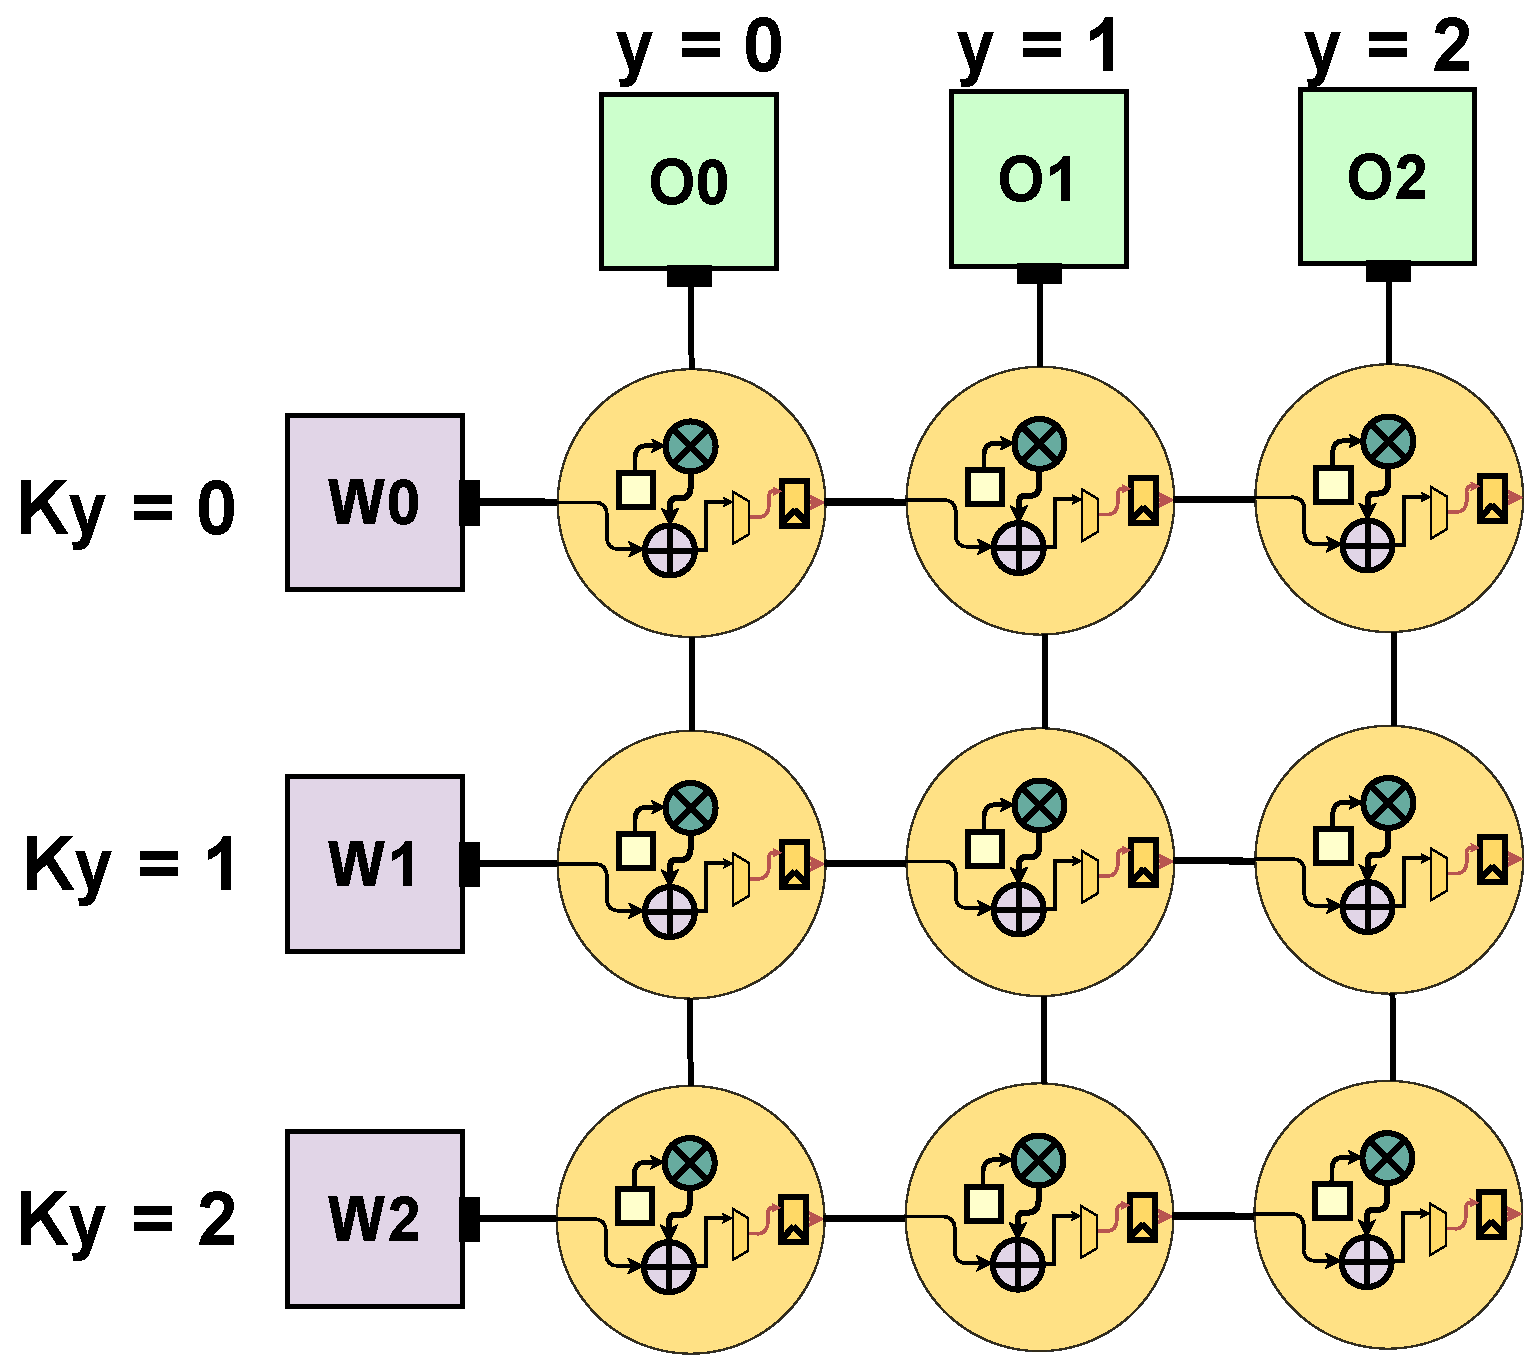
\includegraphics[width=0.32\textwidth]{fig/unroll_fy_y.pdf}}
    \hspace{0.1cm} 
    \subfigure[]{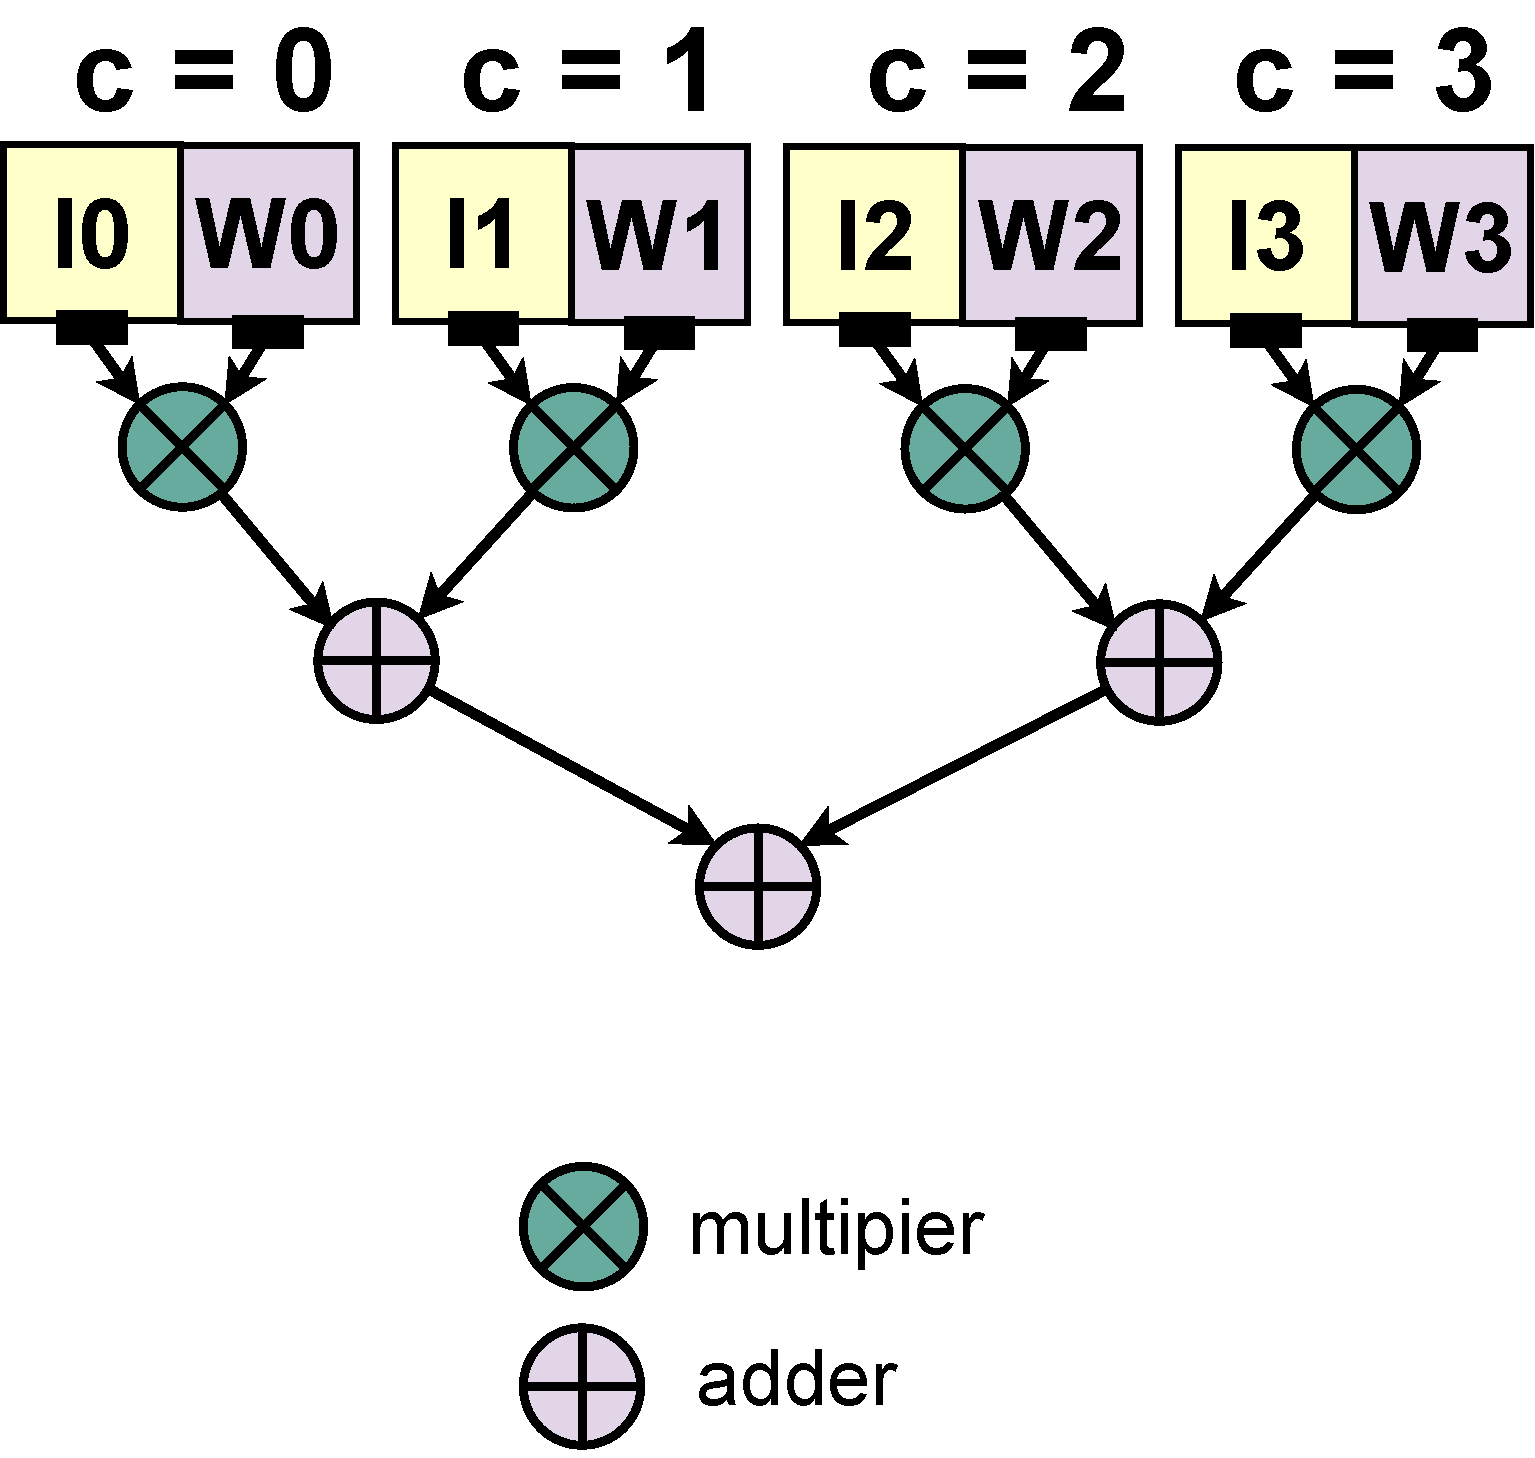
\includegraphics[width=0.32\textwidth]{fig/unroll_c.pdf}} 
    \hspace{0.1cm} 
    \subfigure[]{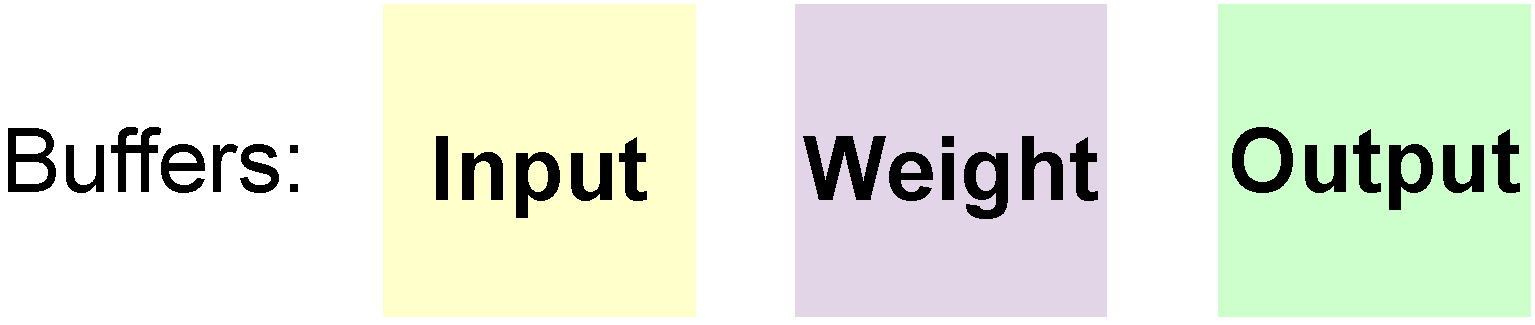
\includegraphics[width=0.3\textwidth]{fig/buffer_description.pdf}}
    \caption{Illustration of different dataflow implementations adapted from \cite{dnn_df_overrated} (a) blah (b) blah (c) blah (d) blah}
    \label{fig:unroll_illustration}
\end{figure}


From dataflow we can derive hw implementation based on communication pattern and
reuse behavior of the individual data elements accessed in the convolution
layer.

\subsection{The Hardware Implementation taxonomy}

Figures in \autoref{fig:unroll_illustration} show different reduction/ multicast
schemes based on reuse behavior of data elements (IFmap, OFmap, Weights)
apparent in the dataflow. The space of available schemes is not limited to those
presented in \autoref{fig:unroll_illustration} though. In \cite{maestro} a
hardware taxonomy illustrated in figure \autoref{fig:hw_taxonpmy}.

\begin{figure}[ht]
    \centering
    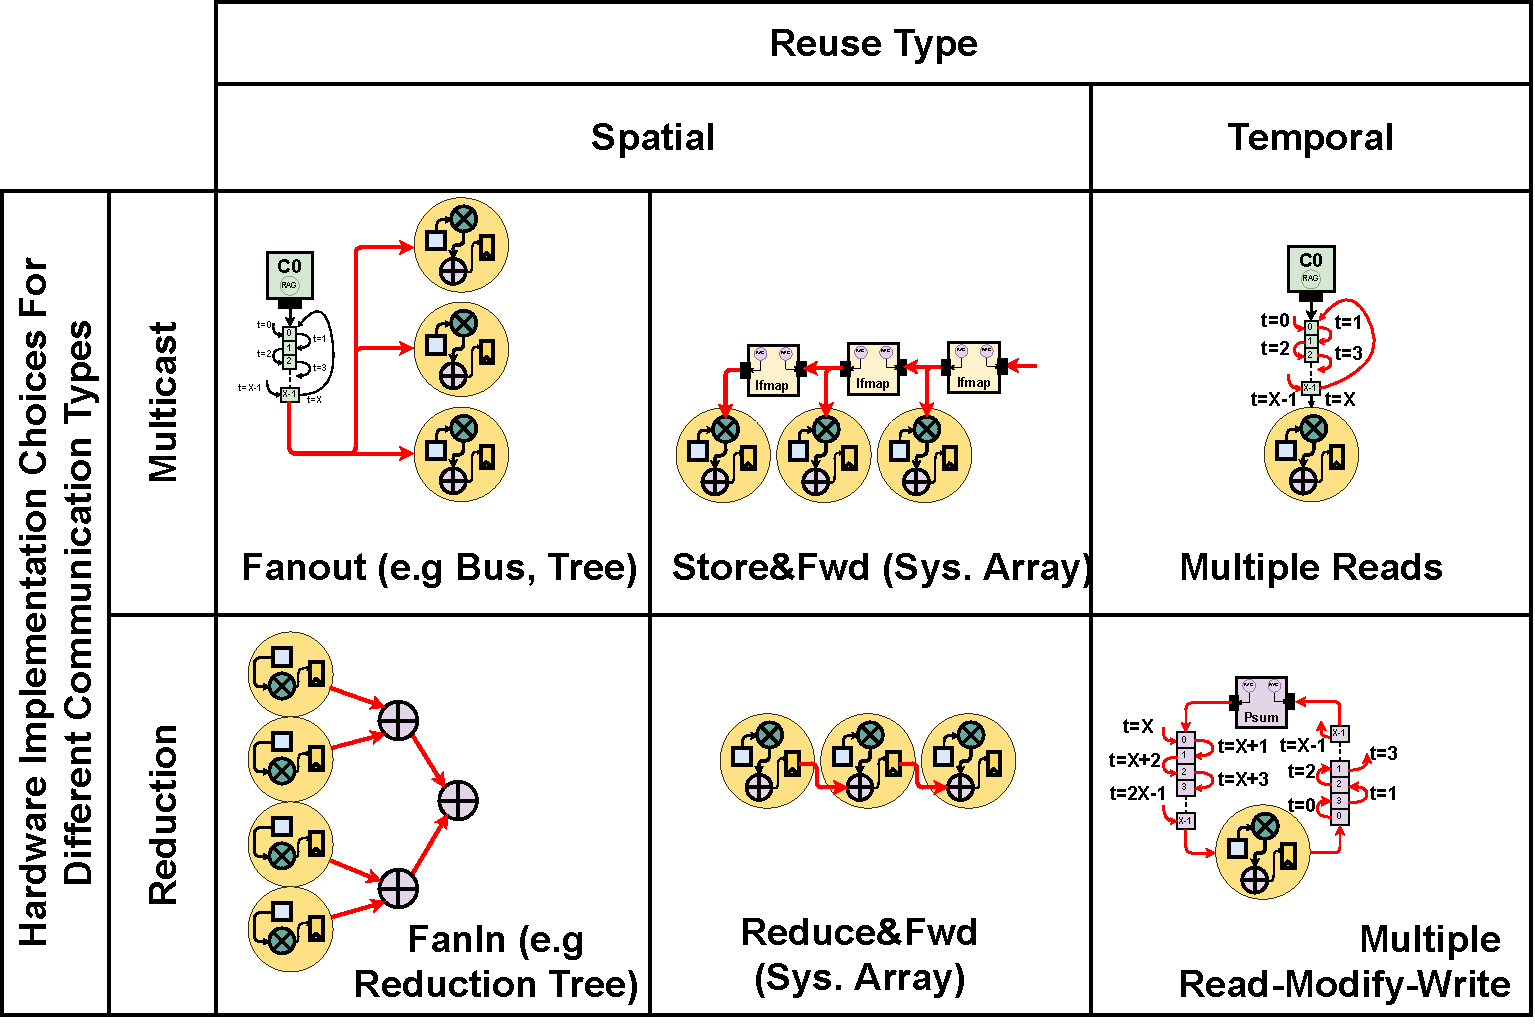
\includegraphics[scale=0.58]{fig/hw_taxonomy.pdf}
    \caption{Hardware Implementation Taxonomy adapted from \cite{maestro}}
    \label{fig:hw_taxonomy}
\end{figure}


Depending on the dataflow described using the dataflow taxonomy (1) loop
ordering (2) unroll targets (2) loop unroll factors. The implementation options
are derived based on the type of reuse present in the dataflow. Following the
hardware implementation taxonomy presented in in \cite{maestro}, we can classify
the available hardware implementation options based on the the type of reuse is
spatial (reuse distance = 0) or temporal (reuse distance > 0) that exists for a
given data element accessed in the dataflow. Within a reuse type, depending on
the nature of the reuse, if it is read or read modify write, there are several
options for supporting the communication inferred from the reuse. To deduce the
type of reuse and overall communicaiton behavior for each data element in any
dataflow we can use the polyhedral model to detect temporal reuse. Spatial reuse
detection can be inferred directly from the loops.


\section{Analysis of data reuse with the polyhedral model}

\cite{meeus} used polyehdral model to analyse reuse within stencil based applications described
as nested loops. One important element in their approach is their program written in iscc that
can determine temporal reuse of data elements

There's the polyhedral extraction tool out there but unfortunately there's no
way to encode parallelism or loop unrolling in it without relying on compiler
pragmas. 

below is an example of this reuse applied to the gemm loops



